\documentclass[12pt, a4paper]{article}
\usepackage{amsmath}
\usepackage{multirow}
\usepackage{multicol}
\usepackage{graphicx}
\title{Report on Soft Soil Improvement Technique}
\author{Jakaria Pervez, Sakib Bin Rafi}
\date{April, 2023}
\begin{document}
\maketitle
Bearing Capacity and Settlement of Natural Ground without improvement:
\[q_{ult}=CN_CS_Cd_C+0.5{\gamma^'}{N_\gamma}{d_\gamma}+{\sigma_D^'}{N_q}{S_q}{d_q}\]\\
\begin{align*}
   \sigma{_D^'} &=(EGL-Foundation Level)*\gamma_{Sub}\\
  & =(1.5-(-)3.35)*\gamma_{Sub}\\
  & =4.85*(15-9.81)\\
  & =4.85*5.19\\
  & =25.2
\end{align*}
Assumed Values\\
$N_\gamma=0, C=5.14, S_C=d_C=1.2, N_q=S_q=d_q=1$

\begin{align*}
\ q_{ult} &=CN_CS_Cd_C+0.5{\gamma^'}{N_\gamma}{d_\gamma}+{\sigma_D^'}{N_q}{S_q}{d_q}\\
  & =37.5*5.14*1.2*1.2+0.5*0*(15-9.81)*1*1+25.2*1*1*1\\
  & =302.76 KPa\\
\end{align*}
\begin{align*}
\ q_{ult,s} &={k^'}{k_p}{C_u}\\\
  & =25*37.5\\
  & =937.5KPa\\
\end{align*}
\begin{align*}
\ q_{ult,req} &=f_s*{Foundation Pressure}\\\
  & =3*120\\
  & =360 KPa\\
\end{align*}
\begin{align*}
\ q_{ult,req} &=q_{ult,c}*a_s+{(1-a_s)}*q_{ult,s}\\\
\ 360 &=937*a_s+{(1-a_s)}*302\\\
\ 360 &=937*a_s-302*a_s+302\\\
\ 360 &=635*a_s+302\\\
\ 635*a_s &=360-302\\\
\ a_s &=\frac{58}{302}\\\
\ a_s &=0.091\\\
\end{align*}
\begin{align*}
\ \frac{s}{d} &=\sqrt\frac{\pi}{4a_s}\\\
  & =\sqrt\frac{3.14}{4*0.091}\\\
  & =2.94\\use,  2.5\\
\end{align*}
Depth of pile= Use 10m Rammed Aggregate Pile with s/d ratio 2.5 and 0.60m Pile dia
\begin{align*}
\ \frac{s}{d} &=2.5\\
\ s  &=2.5*0.6\\\
\ s  &=1.50m\\\
\end{align*}
Total Area= $635m^2$\\
Reduced Area= $a_s*A=0.125*635=80m^2$\\
Area of Pile= $\frac{\pi}{4}*0.6^2=0.282m^2$
No of Pile= $\frac{80}{0.282}=283nos$\\

\textbf{Pile Cost:}\\
Compacted Volume=$\frac{\pi}{4}*d^2*l=0.282*10=2.82m^3$\\
Uncompacted Volume=$ 1.5*2.82=4.23m^3$\\
Khoa Filter:
Code: 40-520-20(40mm to 20mm)-4900.41TK\\
Code: 40-520-30(20mm to 5mm)-5401.45TK\\
Material Cost=4.23*5401.45=22848.13TK\\
Installation Cost= 0.33*22848.13=7539.88TK\\
Cost Per Pile= 22848.13+7539.88= 30388TK= 0.31 Lakh TK/Pile\\
Total Pile Cost= 0.31*283=87.73 Lakh TK
\begin{align*}
    \ Q_{Allowable} &=\frac{173.23}{3}\\
    &= 57.74\\
\end{align*}
Not OK for Bearing Capacity\\
\textbf{Settlement Calculation:}
\[S_C=\frac{C_CH}{1+e_0}log\frac{P_0+\Delta P}{P_0}\]\\
Assumed Values\\
$H=12.80m, e_0=0.25, C_C=0.3$\\
$P_0=6.4*(15-9.81)=33.28$\\
\begin{align*}
\ S_C &=\frac{C_CH}{1+e_0}log\frac{P_0+\Delta P}{P_0}\\
  & =\frac{0.3H}{1+0.25}log\frac{33.28+120}{33.28}\\
  & =0.16H(Maximum)\\
  & =0.1H(Average)\\
  & =0.07H(Minimum)\\
\end{align*}
Minimum Settlement=0.07*12800=905mm\\
\textbf{Settlement Time Factor}
Representative values for $E_S$ and $\mu$ for different types of soil:\\
\begin{table}[ht]
    \centering
    \begin{tabular}{|c|c|c|}
    \hline
    \textbf{SPT} & \textbf{Soil Consistency} & \textbf{$C_uKsf(KPa)$}\\
    \hline
    $<2$ & Very Soft & $0.4(20)$\\
    \hline
    $2-4$ & Soft & $0.4-0.8(20-40)$\\
    \hline
    $4-8$ & Firm & $0.8-1.5(40-75)$\\
    \hline
    $8-15$ & Stiff & $1.5-3(75-150)$\\
    \hline
    $15-30$ & Very Stiff & $3-6(150-300)$\\
    \hline
    $>30$ & Hard & \\
    \hline
    \end{tabular}
    \caption{SPT Correlation of Cohessive Soil}
    \label{tab:my_label}
\end{table}
\begin{table}[ht]
    \centering
    \begin{tabular}{|c|c|}
    \hline
    \textbf{Soil Type} & \textbf{Poissons's Ratio, $\mu$}\\
    \hline
    Loose Sand & 0.2-0.4\\
    \hline
    Medium Sand & 0.25-0.4\\
    \hline
    Dense Sand & 0.3-0.45\\
    \hline
    Silty Sand & 0.2-0.4\\
    \hline
    Soft Clay & 0.15-0.25\\
    \hline
    Medium Clay & 0.2-0\\
    \hline
    Silty Sand & 0.2-0.4\\
    \hline
    \end{tabular}
    \caption{Table 11.4 [Source: BM Das, Page- 302]}
    \label{tab:my_label}
\end{table}\\
Coefficient of Volumetric Compressibility, \[m_V=\frac{(1+\mu_S)(1-2\mu_S)}{E_S(1-\mu_S}\]
Time Factor, \[T_V=\frac{C_Vt}{H^2_{dr}}\]
Coefficient of Vertical Permeability, \[C_V=\frac{k}{\gamma_wm_v}\]
Where, K=Coefficient of Permeability\\

\begin{figure}
    \centering
    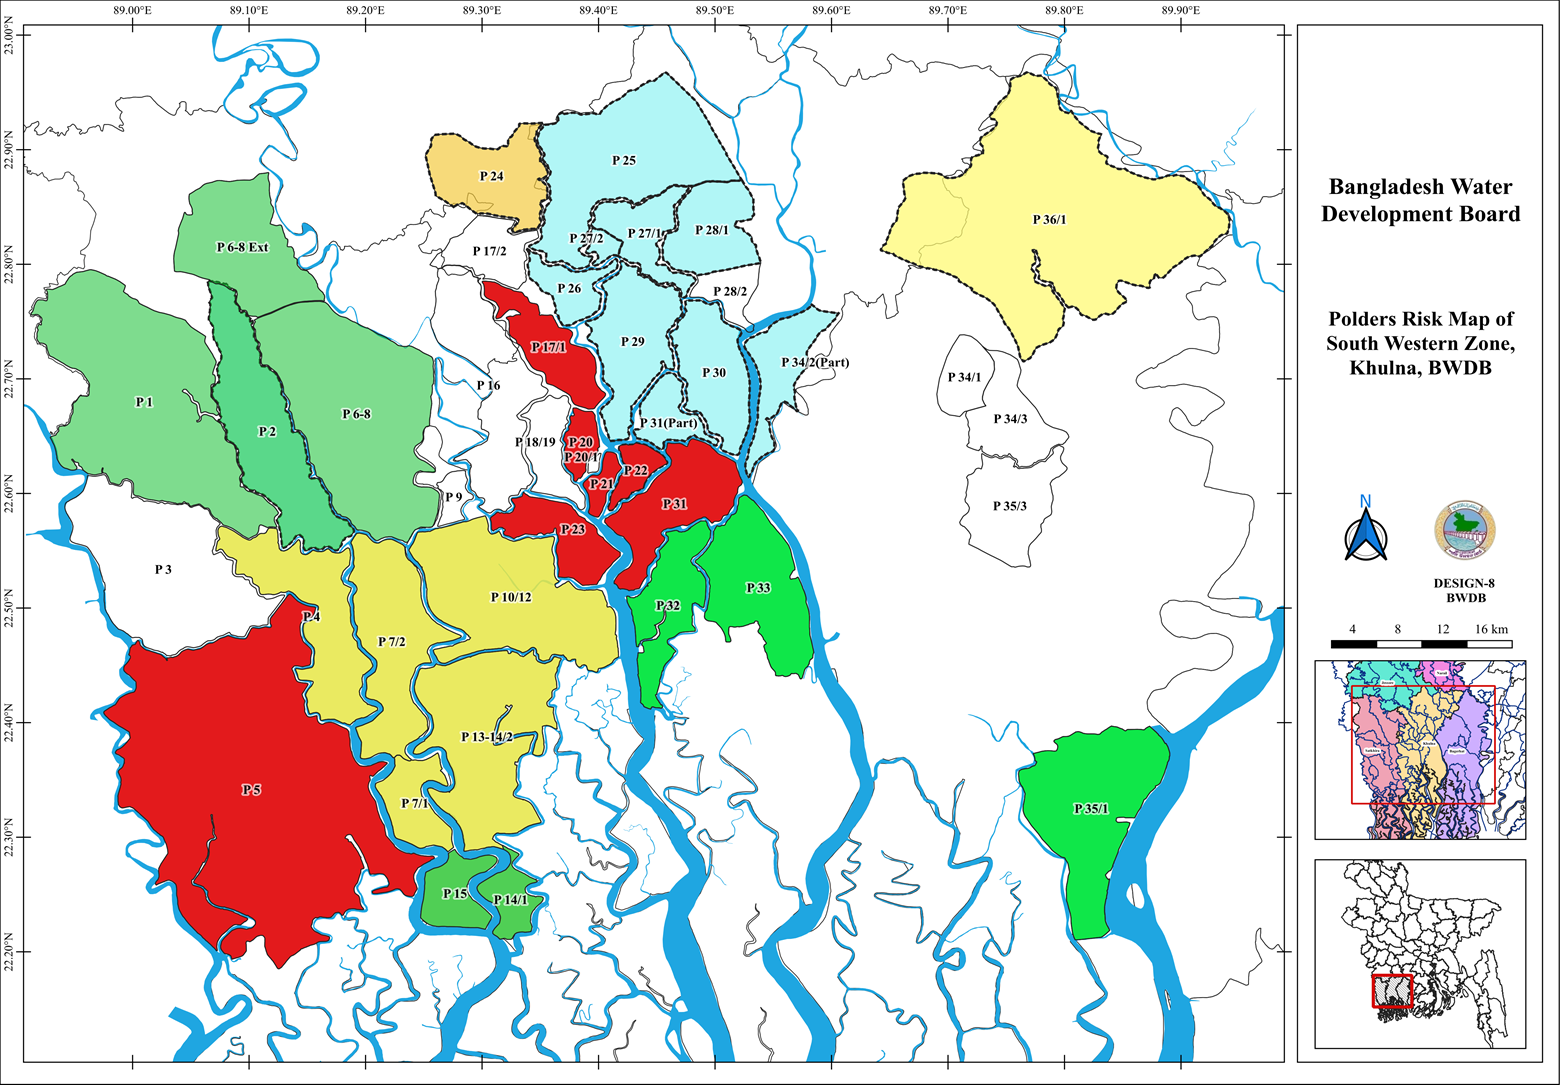
\includegraphics[width=\linewidth]{noname.png}
    \caption{figure-1}
    \label{fig:my_label}     
\end{figure}
\end{document}

 